% ============================================================
% Question Bank: ch06-06 Angle Relationships
% Topic Title: Angle Relationships: Supplementary, Complementary, and Vertical Angles
% CCSS: 7.G.B.5
% Questions: 27 (15 MC + 6 SA + 6 Graphical)
% ============================================================

% --- Multiple Choice Questions (15) ---

\begin{practiceQuestion}{6-6-q01}{mc}
\begin{questionText}
Two angles are supplementary. One angle measures $128°$. What is the measure of the other angle?
\end{questionText}
\choiceA{$32°$}
\choiceB{$52°$}
\choiceC{$62°$}
\choiceD{$128°$}
\correctAnswer{B}
\explanation{Supplementary angles sum to $180°$. The other angle is $180° - 128° = 52°$.}
\end{practiceQuestion}

\begin{practiceQuestion}{6-6-q02}{mc}
\begin{questionText}
Two angles are complementary. One angle measures $34°$. What is the measure of the other angle?
\end{questionText}
\choiceA{$34°$}
\choiceB{$46°$}
\choiceC{$56°$}
\choiceD{$146°$}
\correctAnswer{C}
\explanation{Complementary angles sum to $90°$. The other angle is $90° - 34° = 56°$.}
\end{practiceQuestion}

\begin{practiceQuestion}{6-6-q03}{mc}
\begin{questionText}
Two lines intersect and one of the angles formed measures $105°$. What is the measure of the angle vertical to it?
\end{questionText}
\choiceA{$75°$}
\choiceB{$85°$}
\choiceC{$105°$}
\choiceD{$180°$}
\correctAnswer{C}
\explanation{Vertical angles are the opposite angles formed when two lines cross; they are always equal. If one angle is $105°$, the vertical angle is also $105°$.}
\end{practiceQuestion}

\begin{practiceQuestion}{6-6-q04}{mc}
\begin{questionText}
Two supplementary angles are $(3x + 5)°$ and $(2x + 25)°$. What is the value of $x$?
\end{questionText}
\choiceA{$25$}
\choiceB{$30$}
\choiceC{$35$}
\choiceD{$40$}
\correctAnswer{B}
\explanation{Supplementary angles sum to $180°$: $(3x + 5) + (2x + 25) = 180$. Combine: $5x + 30 = 180$. Subtract $30$: $5x = 150$. Divide: $x = 30$.}
\end{practiceQuestion}

\begin{practiceQuestion}{6-6-q05}{mc}
\begin{questionText}
Two complementary angles are $(x + 8)°$ and $(3x - 2)°$. What is the measure of the larger angle?
\end{questionText}
\choiceA{$29°$}
\choiceB{$42°$}
\choiceC{$48°$}
\choiceD{$61°$}
\correctAnswer{D}
\explanation{Complementary angles sum to $90°$: $(x + 8) + (3x - 2) = 90$. Combine: $4x + 6 = 90$. Solve: $4x = 84$, $x = 21$. The angles are $21 + 8 = 29°$ and $3(21) - 2 = 61°$. The larger is $61°$.}
\end{practiceQuestion}

\begin{practiceQuestion}{6-6-q06}{mc}
\begin{questionText}
Which pair of angles are complementary?
\end{questionText}
\choiceA{$55°$ and $125°$}
\choiceB{$37°$ and $53°$}
\choiceC{$90°$ and $90°$}
\choiceD{$45°$ and $135°$}
\correctAnswer{B}
\explanation{Complementary angles sum to $90°$. Testing each: $55 + 125 = 180$, $37 + 53 = 90$ \checkmark, $90 + 90 = 180$, $45 + 135 = 180$. Only choice B sums to $90°$.}
\end{practiceQuestion}

\begin{practiceQuestion}{6-6-q07}{mc}
\begin{questionText}
Two vertical angles are $(4x + 10)°$ and $(6x - 20)°$. What is the measure of each angle?
\end{questionText}
\choiceA{$50°$}
\choiceB{$60°$}
\choiceC{$70°$}
\choiceD{$80°$}
\correctAnswer{C}
\explanation{Vertical angles are equal: $4x + 10 = 6x - 20$. Subtract $4x$: $10 = 2x - 20$. Add $20$: $30 = 2x$. Divide: $x = 15$. Each angle is $4(15) + 10 = 70°$.}
\end{practiceQuestion}

\begin{practiceQuestion}{6-6-q08}{mc}
\begin{questionText}
An angle measures $73°$. What is the measure of its supplement?
\end{questionText}
\choiceA{$17°$}
\choiceB{$73°$}
\choiceC{$107°$}
\choiceD{$117°$}
\correctAnswer{C}
\explanation{Supplementary angles sum to $180°$. The supplement is $180° - 73° = 107°$.}
\end{practiceQuestion}

\begin{practiceQuestion}{6-6-q09}{mc}
\begin{questionText}
Two adjacent angles on a straight line are $(5x)°$ and $(4x)°$. What is the value of $x$?
\end{questionText}
\choiceA{$10$}
\choiceB{$15$}
\choiceC{$20$}
\choiceD{$36$}
\correctAnswer{C}
\explanation{Adjacent angles on a straight line are supplementary (sum to $180°$): $5x + 4x = 180$. Combine: $9x = 180$. Divide: $x = 20$.}
\end{practiceQuestion}

\begin{practiceQuestion}{6-6-q10}{mc}
\begin{questionText}
Three angles meet at a point on a line. Their measures are $x°$, $55°$, and $75°$. What is the value of $x$?
\end{questionText}
\choiceA{$40°$}
\choiceB{$50°$}
\choiceC{$60°$}
\choiceD{$130°$}
\correctAnswer{B}
\explanation{Angles on one side of a straight line sum to $180°$. So $x + 55 + 75 = 180$, which gives $x + 130 = 180$, and $x = 50°$.}
\end{practiceQuestion}

\begin{practiceQuestion}{6-6-q11}{mc}
\begin{questionText}
Angle $A$ and Angle $B$ are vertical angles. Angle $A = (2x + 40)°$ and Angle $B = (4x)°$. What is the measure of Angle $A$?
\end{questionText}
\choiceA{$20°$}
\choiceB{$40°$}
\choiceC{$60°$}
\choiceD{$80°$}
\correctAnswer{D}
\explanation{Vertical angles are equal: $2x + 40 = 4x$. Subtract $2x$: $40 = 2x$, so $x = 20$. Angle $A = 2(20) + 40 = 80°$.}
\end{practiceQuestion}

\begin{practiceQuestion}{6-6-q12}{mc}
\begin{questionText}
Which statement is always true?
\end{questionText}
\choiceA{Complementary angles are always adjacent}
\choiceB{Vertical angles are supplementary}
\choiceC{Vertical angles are congruent}
\choiceD{Supplementary angles are always right angles}
\correctAnswer{C}
\explanation{By the vertical angles theorem, vertical angles (formed by two intersecting lines) are always congruent (equal in measure). The other statements are not always true.}
\end{practiceQuestion}

\begin{practiceQuestion}{6-6-q13}{mc}
\begin{questionText}
An angle is $15°$ more than twice its complement. What is the measure of the angle?
\end{questionText}
\choiceA{$25°$}
\choiceB{$55°$}
\choiceC{$65°$}
\choiceD{$75°$}
\correctAnswer{C}
\explanation{Let the angle be $x$ and its complement be $90 - x$. Then $x = 2(90 - x) + 15$. Expand: $x = 180 - 2x + 15 = 195 - 2x$. Add $2x$: $3x = 195$. Divide: $x = 65°$.}
\end{practiceQuestion}

\begin{practiceQuestion}{6-6-q14}{mc}
\begin{questionText}
Two angles form a linear pair. One angle is $5$ times the other. What are the two angle measures?
\end{questionText}
\choiceA{$15°$ and $75°$}
\choiceB{$20°$ and $100°$}
\choiceC{$30°$ and $150°$}
\choiceD{$36°$ and $144°$}
\correctAnswer{C}
\explanation{A linear pair sums to $180°$. Let the smaller angle be $x$: $x + 5x = 180$, so $6x = 180$ and $x = 30°$. The angles are $30°$ and $150°$.}
\end{practiceQuestion}

\begin{practiceQuestion}{6-6-q15}{mc}
\begin{questionText}
A right angle is divided into two parts by a ray. One part measures $(2x + 5)°$ and the other measures $(x + 1)°$. What is the value of $x$?
\end{questionText}
\choiceA{$24$}
\choiceB{$28$}
\choiceC{$30$}
\choiceD{$42$}
\correctAnswer{B}
\explanation{The two parts of a right angle sum to $90°$: $(2x + 5) + (x + 1) = 90$. Combine: $3x + 6 = 90$. Subtract $6$: $3x = 84$. Divide: $x = 28$.}
\end{practiceQuestion}

% --- Short Answer Questions (6) ---

\begin{practiceQuestion}{6-6-q16}{sa}
\begin{questionText}
An angle measures $47°$. Find both its complement and its supplement.
\end{questionText}
\correctAnswer{Complement: $43°$; Supplement: $133°$}
\explanation{The complement is $90° - 47° = 43°$. The supplement is $180° - 47° = 133°$.}
\end{practiceQuestion}

\begin{practiceQuestion}{6-6-q17}{sa}
\begin{questionText}
Two vertical angles are $(7x - 5)°$ and $(5x + 19)°$. Find the measure of each angle.
\end{questionText}
\correctAnswer{$79°$}
\explanation{Vertical angles are equal: $7x - 5 = 5x + 19$. Subtract $5x$: $2x - 5 = 19$. Add $5$: $2x = 24$, so $x = 12$. Each angle is $7(12) - 5 = 79°$.}
\end{practiceQuestion}

\begin{practiceQuestion}{6-6-q18}{sa}
\begin{questionText}
Two supplementary angles are in the ratio $5:4$. What are the measures of the two angles?
\end{questionText}
\correctAnswer{$100°$ and $80°$}
\explanation{Let the angles be $5k$ and $4k$. Then $5k + 4k = 180$, so $9k = 180$ and $k = 20$. The angles are $5(20) = 100°$ and $4(20) = 80°$.}
\end{practiceQuestion}

\begin{practiceQuestion}{6-6-q19}{sa}
\begin{questionText}
Three angles meet at a point. Two of the angles measure $110°$ and $95°$. What is the third angle?
\end{questionText}
\correctAnswer{$155°$}
\explanation{Angles around a point sum to $360°$. The third angle is $360° - 110° - 95° = 155°$.}
\end{practiceQuestion}

\begin{practiceQuestion}{6-6-q20}{sa}
\begin{questionText}
An angle is $20°$ less than three times its supplement. Find the measure of the angle.
\end{questionText}
\correctAnswer{$130°$}
\explanation{Let the angle be $x$ and its supplement be $180 - x$. Then $x = 3(180 - x) - 20$. Expand: $x = 540 - 3x - 20 = 520 - 3x$. Add $3x$: $4x = 520$. Divide: $x = 130°$.}
\end{practiceQuestion}

\begin{practiceQuestion}{6-6-q21}{sa}
\begin{questionText}
Two complementary angles are in the ratio $2:7$. What is the measure of the larger angle?
\end{questionText}
\correctAnswer{$70°$}
\explanation{Let the angles be $2k$ and $7k$. Then $2k + 7k = 90$, so $9k = 90$ and $k = 10$. The larger angle is $7(10) = 70°$.}
\end{practiceQuestion}

% --- Graphical MC Questions (3) ---

\begin{practiceQuestion}{6-6-q22}{gmc}
\begin{questionText}
In the diagram below, two straight lines intersect. Find the value of $x$.

\begin{center}
\begin{tikzpicture}[scale=0.9]
  \draw[thick] (-3,0) -- (3,0);
  \draw[thick] (-2,-2) -- (2,2);
  \node at (1.3,0.4) {$x°$};
  \node at (-1.5,-0.5) {$135°$};
\end{tikzpicture}
\end{center}
\end{questionText}
\choiceA{$35°$}
\choiceB{$45°$}
\choiceC{$55°$}
\choiceD{$135°$}
\correctAnswer{B}
\explanation{The angle labeled $135°$ and the angle $x°$ are supplementary because they form a linear pair on a straight line. So $x = 180° - 135° = 45°$.}
\end{practiceQuestion}

\begin{practiceQuestion}{6-6-q23}{gmc}
\begin{questionText}
In the figure below, $\angle AOB$ and $\angle BOC$ are complementary. Find the value of $x$.

\begin{center}
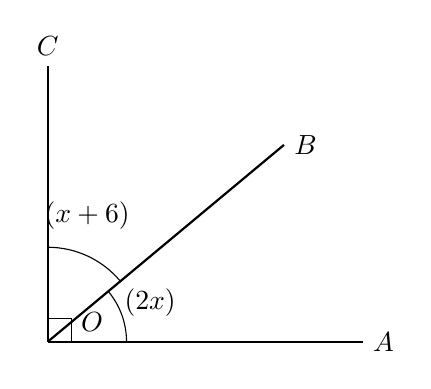
\begin{tikzpicture}[scale=1.0]
  \draw[thick] (0,0) -- (4,0) node[right] {$A$};
  \draw[thick] (0,0) -- (3,2.5) node[right] {$B$};
  \draw[thick] (0,0) -- (0,3.5) node[above] {$C$};
  \node at (0.3,0) [above right] {$O$};
  % Angle AOB
  \draw (1,0) arc[start angle=0,end angle=40,radius=1];
  \node at (1.3,0.5) {$(2x)°$};
  % Angle BOC
  \draw (0,1.2) arc[start angle=90,end angle=40,radius=1.2];
  \node at (0.5,1.6) {$(x+6)°$};
  % Right angle mark
  \draw (0.3,0) -- (0.3,0.3) -- (0,0.3);
\end{tikzpicture}
\end{center}
\end{questionText}
\choiceA{$24$}
\choiceB{$28$}
\choiceC{$32$}
\choiceD{$36$}
\correctAnswer{B}
\explanation{Since $\angle AOC = 90°$, the two angles are complementary: $2x + (x + 6) = 90$. Combine: $3x + 6 = 90$. Subtract $6$: $3x = 84$. Divide: $x = 28$.}
\end{practiceQuestion}

\begin{practiceQuestion}{6-6-q24}{gmc}
\begin{questionText}
Two lines intersect as shown below. What is the value of $y$?

\begin{center}
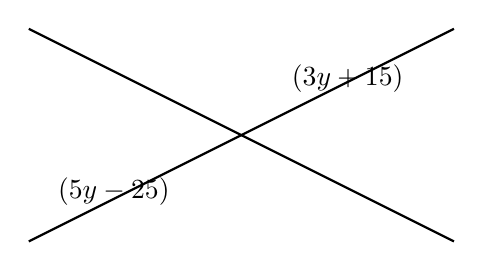
\begin{tikzpicture}[scale=0.9]
  \draw[thick] (-3,-1.5) -- (3,1.5);
  \draw[thick] (-3,1.5) -- (3,-1.5);
  \node at (1.5,0.8) {$(3y + 15)°$};
  \node at (-1.8,-0.8) {$(5y - 25)°$};
\end{tikzpicture}
\end{center}
\end{questionText}
\choiceA{$10$}
\choiceB{$15$}
\choiceC{$20$}
\choiceD{$25$}
\correctAnswer{C}
\explanation{The two labeled angles are vertical angles, so they are equal: $3y + 15 = 5y - 25$. Subtract $3y$: $15 = 2y - 25$. Add $25$: $40 = 2y$. Divide: $y = 20$.}
\end{practiceQuestion}

% --- Graphical SA Questions (3) ---

\begin{practiceQuestion}{6-6-q25}{gsa}
\begin{questionText}
In the diagram below, lines $\ell$ and $m$ intersect at point $P$. Find the measures of angles $a$, $b$, and $c$.

\begin{center}
\begin{tikzpicture}[scale=0.9]
  \draw[thick] (-3,0) -- (3,0) node[right] {$\ell$};
  \draw[thick] (-2,-2.5) -- (2,2.5) node[right] {$m$};
  \node at (0,-0.3) {$P$};
  \node at (1.2,0.5) {$a$};
  \node at (-0.8,0.5) {$58°$};
  \node at (-1.2,-0.5) {$b$};
  \node at (0.8,-0.5) {$c$};
\end{tikzpicture}
\end{center}
\end{questionText}
\correctAnswer{$a = 122°$, $b = 58°$, $c = 122°$}
\explanation{Angle $a$ and the $58°$ angle are supplementary (linear pair): $a = 180° - 58° = 122°$. Angle $b$ is vertical to the $58°$ angle, so $b = 58°$. Angle $c$ is vertical to angle $a$, so $c = 122°$.}
\end{practiceQuestion}

\begin{practiceQuestion}{6-6-q26}{gsa}
\begin{questionText}
In the figure below, angles $1$ and $2$ are complementary. If $\angle 1 = (4n - 3)°$ and $\angle 2 = (2n + 9)°$, find $n$ and the measure of each angle.

\begin{center}
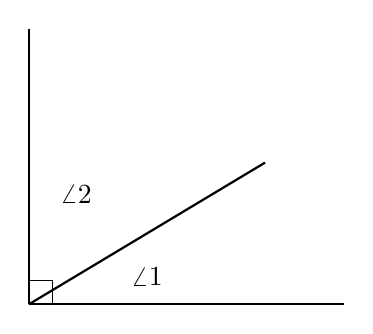
\begin{tikzpicture}[scale=1.0]
  \draw[thick] (0,0) -- (4,0);
  \draw[thick] (0,0) -- (3,1.8);
  \draw[thick] (0,0) -- (0,3.5);
  % Right angle
  \draw (0.3,0) -- (0.3,0.3) -- (0,0.3);
  % Labels
  \node at (1.5,0.35) {$\angle 1$};
  \node at (0.6,1.4) {$\angle 2$};
\end{tikzpicture}
\end{center}
\end{questionText}
\correctAnswer{$n = 14$; $\angle 1 = 53°$, $\angle 2 = 37°$}
\explanation{Complementary angles sum to $90°$: $(4n - 3) + (2n + 9) = 90$. Combine: $6n + 6 = 90$. Subtract $6$: $6n = 84$. Divide: $n = 14$. Then $\angle 1 = 4(14) - 3 = 53°$ and $\angle 2 = 2(14) + 9 = 37°$.}
\end{practiceQuestion}

\begin{practiceQuestion}{6-6-q27}{gsa}
\begin{questionText}
In the diagram, two straight lines cross. Find the values of $x$ and $y$.

\begin{center}
\begin{tikzpicture}[scale=0.9]
  \draw[thick] (-3,0) -- (3,0);
  \draw[thick] (-1.5,-2.5) -- (1.5,2.5);
  \node at (1,0.7) {$(2x + 10)°$};
  \node at (-1.3,-0.7) {$(3x - 20)°$};
  \node at (-1.3,0.5) {$y°$};
\end{tikzpicture}
\end{center}
\end{questionText}
\correctAnswer{$x = 30$; $y = 110°$}
\explanation{The angles $(2x + 10)°$ and $(3x - 20)°$ are vertical angles, so $2x + 10 = 3x - 20$. Subtract $2x$: $10 = x - 20$. Add $20$: $x = 30$. The vertical angle is $2(30) + 10 = 70°$. Since $y$ and $70°$ form a linear pair: $y = 180° - 70° = 110°$.}
\end{practiceQuestion}
